\documentclass[twoside]{book}

% Packages required by doxygen
\usepackage{fixltx2e}
\usepackage{calc}
\usepackage{doxygen}
\usepackage[export]{adjustbox} % also loads graphicx
\usepackage{graphicx}
\usepackage[utf8]{inputenc}
\usepackage{makeidx}
\usepackage{multicol}
\usepackage{multirow}
\PassOptionsToPackage{warn}{textcomp}
\usepackage{textcomp}
\usepackage[nointegrals]{wasysym}
\usepackage[table]{xcolor}

% Font selection
\usepackage[T1]{fontenc}
\usepackage[scaled=.90]{helvet}
\usepackage{courier}
\usepackage{amssymb}
\usepackage{sectsty}
\renewcommand{\familydefault}{\sfdefault}
\allsectionsfont{%
  \fontseries{bc}\selectfont%
  \color{darkgray}%
}
\renewcommand{\DoxyLabelFont}{%
  \fontseries{bc}\selectfont%
  \color{darkgray}%
}
\newcommand{\+}{\discretionary{\mbox{\scriptsize$\hookleftarrow$}}{}{}}

% Page & text layout
\usepackage{geometry}
\geometry{%
  a4paper,%
  top=2.5cm,%
  bottom=2.5cm,%
  left=2.5cm,%
  right=2.5cm%
}
\tolerance=750
\hfuzz=15pt
\hbadness=750
\setlength{\emergencystretch}{15pt}
\setlength{\parindent}{0cm}
\setlength{\parskip}{3ex plus 2ex minus 2ex}
\makeatletter
\renewcommand{\paragraph}{%
  \@startsection{paragraph}{4}{0ex}{-1.0ex}{1.0ex}{%
    \normalfont\normalsize\bfseries\SS@parafont%
  }%
}
\renewcommand{\subparagraph}{%
  \@startsection{subparagraph}{5}{0ex}{-1.0ex}{1.0ex}{%
    \normalfont\normalsize\bfseries\SS@subparafont%
  }%
}
\makeatother

% Headers & footers
\usepackage{fancyhdr}
\pagestyle{fancyplain}
\fancyhead[LE]{\fancyplain{}{\bfseries\thepage}}
\fancyhead[CE]{\fancyplain{}{}}
\fancyhead[RE]{\fancyplain{}{\bfseries\leftmark}}
\fancyhead[LO]{\fancyplain{}{\bfseries\rightmark}}
\fancyhead[CO]{\fancyplain{}{}}
\fancyhead[RO]{\fancyplain{}{\bfseries\thepage}}
\fancyfoot[LE]{\fancyplain{}{}}
\fancyfoot[CE]{\fancyplain{}{}}
\fancyfoot[RE]{\fancyplain{}{\bfseries\scriptsize Generated by Doxygen }}
\fancyfoot[LO]{\fancyplain{}{\bfseries\scriptsize Generated by Doxygen }}
\fancyfoot[CO]{\fancyplain{}{}}
\fancyfoot[RO]{\fancyplain{}{}}
\renewcommand{\footrulewidth}{0.4pt}
\renewcommand{\chaptermark}[1]{%
  \markboth{#1}{}%
}
\renewcommand{\sectionmark}[1]{%
  \markright{\thesection\ #1}%
}

% Indices & bibliography
\usepackage{natbib}
\usepackage[titles]{tocloft}
\setcounter{tocdepth}{3}
\setcounter{secnumdepth}{5}
\makeindex

% Hyperlinks (required, but should be loaded last)
\usepackage{ifpdf}
\ifpdf
  \usepackage[pdftex,pagebackref=true]{hyperref}
\else
  \usepackage[ps2pdf,pagebackref=true]{hyperref}
\fi
\hypersetup{%
  colorlinks=true,%
  linkcolor=blue,%
  citecolor=blue,%
  unicode%
}

% Custom commands
\newcommand{\clearemptydoublepage}{%
  \newpage{\pagestyle{empty}\cleardoublepage}%
}

\usepackage{caption}
\captionsetup{labelsep=space,justification=centering,font={bf},singlelinecheck=off,skip=4pt,position=top}

%===== C O N T E N T S =====

\begin{document}

% Titlepage & ToC
\hypersetup{pageanchor=false,
             bookmarksnumbered=true,
             pdfencoding=unicode
            }
\pagenumbering{alph}
\begin{titlepage}
\vspace*{7cm}
\begin{center}%
{\Large My Project \\[1ex]\large 0.\+2 }\\
\vspace*{1cm}
{\large Generated by Doxygen 1.8.13}\\
\end{center}
\end{titlepage}
\clearemptydoublepage
\pagenumbering{roman}
\tableofcontents
\clearemptydoublepage
\pagenumbering{arabic}
\hypersetup{pageanchor=true}

%--- Begin generated contents ---
\chapter{final\+\_\+project}
\label{md__home_ashutosh_catkin_ws_src_final_project__r_e_a_d_m_e}
\Hypertarget{md__home_ashutosh_catkin_ws_src_final_project__r_e_a_d_m_e}
Non-\/complete package for the final project for\+: E\+N\+P\+M809Y Fall 2021


\begin{DoxyItemize}
\item The {\ttfamily doc} folder contains the instructions.
\item The {\ttfamily script} folder contains install.\+bash to install required packages. 
\end{DoxyItemize}
\chapter{text}
\label{md__home_ashutosh_catkin_ws_src_final_project_text}
\Hypertarget{md__home_ashutosh_catkin_ws_src_final_project_text}
Teamp members\+: Sri Sai Charan Velisetti (117509755) Mukundan 
\chapter{Class Index}
\section{Class List}
Here are the classes, structs, unions and interfaces with brief descriptions\+:\begin{DoxyCompactList}
\item\contentsline{section}{\hyperlink{classpath}{path} \\*Creating a object of arrays that are used to store the x and y cordinates of the the follower and explorer }{\pageref{classpath}}{}
\end{DoxyCompactList}

\chapter{File Index}
\section{File List}
Here is a list of all documented files with brief descriptions\+:\begin{DoxyCompactList}
\item\contentsline{section}{/home/ashutosh/catkin\+\_\+ws/src/final\+\_\+project/header/{\bfseries data.\+h} }{\pageref{data_8h}}{}
\item\contentsline{section}{/home/ashutosh/catkin\+\_\+ws/src/final\+\_\+project/src/\hyperlink{main_8cpp}{main.\+cpp} \\*The aim of the project is Urban Search \& Rescue by executing the individual tasks of navigating the explorer and follower robots in the given map }{\pageref{main_8cpp}}{}
\end{DoxyCompactList}

\chapter{Class Documentation}
\hypertarget{classpath}{}\section{path Class Reference}
\label{classpath}\index{path@{path}}


Creating a object of arrays that are used to store the x and y cordinates of the the follower and explorer.  




{\ttfamily \#include $<$data.\+h$>$}

\subsection*{Public Attributes}
\begin{DoxyCompactItemize}
\item 
\mbox{\Hypertarget{classpath_ac6264a569f37ab849f6f3975e8a7ba37}\label{classpath_ac6264a569f37ab849f6f3975e8a7ba37}} 
double {\bfseries x\+\_\+cord} = 0
\item 
\mbox{\Hypertarget{classpath_a4b52cdc69eb3e91576d343b1539aa3e3}\label{classpath_a4b52cdc69eb3e91576d343b1539aa3e3}} 
double {\bfseries y\+\_\+cord} = 0
\item 
\mbox{\Hypertarget{classpath_a52894d0a8d7869c50aeca8a532d34437}\label{classpath_a52894d0a8d7869c50aeca8a532d34437}} 
int {\bfseries f\+\_\+id} = 0
\end{DoxyCompactItemize}


\subsection{Detailed Description}
Creating a object of arrays that are used to store the x and y cordinates of the the follower and explorer. 

Definition at line 16 of file data.\+h.



The documentation for this class was generated from the following file\+:\begin{DoxyCompactItemize}
\item 
/home/ashutosh/catkin\+\_\+ws/src/final\+\_\+project/header/data.\+h\end{DoxyCompactItemize}

\chapter{File Documentation}
\hypertarget{main_8cpp}{}\section{/home/ashutosh/catkin\+\_\+ws/src/final\+\_\+project/src/main.cpp File Reference}
\label{main_8cpp}\index{/home/ashutosh/catkin\+\_\+ws/src/final\+\_\+project/src/main.\+cpp@{/home/ashutosh/catkin\+\_\+ws/src/final\+\_\+project/src/main.\+cpp}}


The aim of the project is Urban Search \& Rescue by executing the individual tasks of navigating the explorer and follower robots in the given map.  


{\ttfamily \#include $<$actionlib/client/simple\+\_\+action\+\_\+client.\+h$>$}\newline
{\ttfamily \#include $<$fiducial\+\_\+msgs/\+Fiducial\+Transform\+Array.\+h$>$}\newline
{\ttfamily \#include $<$geometry\+\_\+msgs/\+Twist.\+h$>$}\newline
{\ttfamily \#include $<$move\+\_\+base\+\_\+msgs/\+Move\+Base\+Action.\+h$>$}\newline
{\ttfamily \#include $<$tf2/\+Linear\+Math/\+Quaternion.\+h$>$}\newline
{\ttfamily \#include $<$tf2\+\_\+ros/transform\+\_\+broadcaster.\+h$>$}\newline
{\ttfamily \#include $<$tf2\+\_\+ros/transform\+\_\+listener.\+h$>$}\newline
{\ttfamily \#include $<$ros/ros.\+h$>$}\newline
{\ttfamily \#include $<$std\+\_\+msgs/\+String.\+h$>$}\newline
{\ttfamily \#include \char`\"{}../header/data.\+h\char`\"{}}\newline
Include dependency graph for main.\+cpp\+:\nopagebreak
\begin{figure}[H]
\begin{center}
\leavevmode
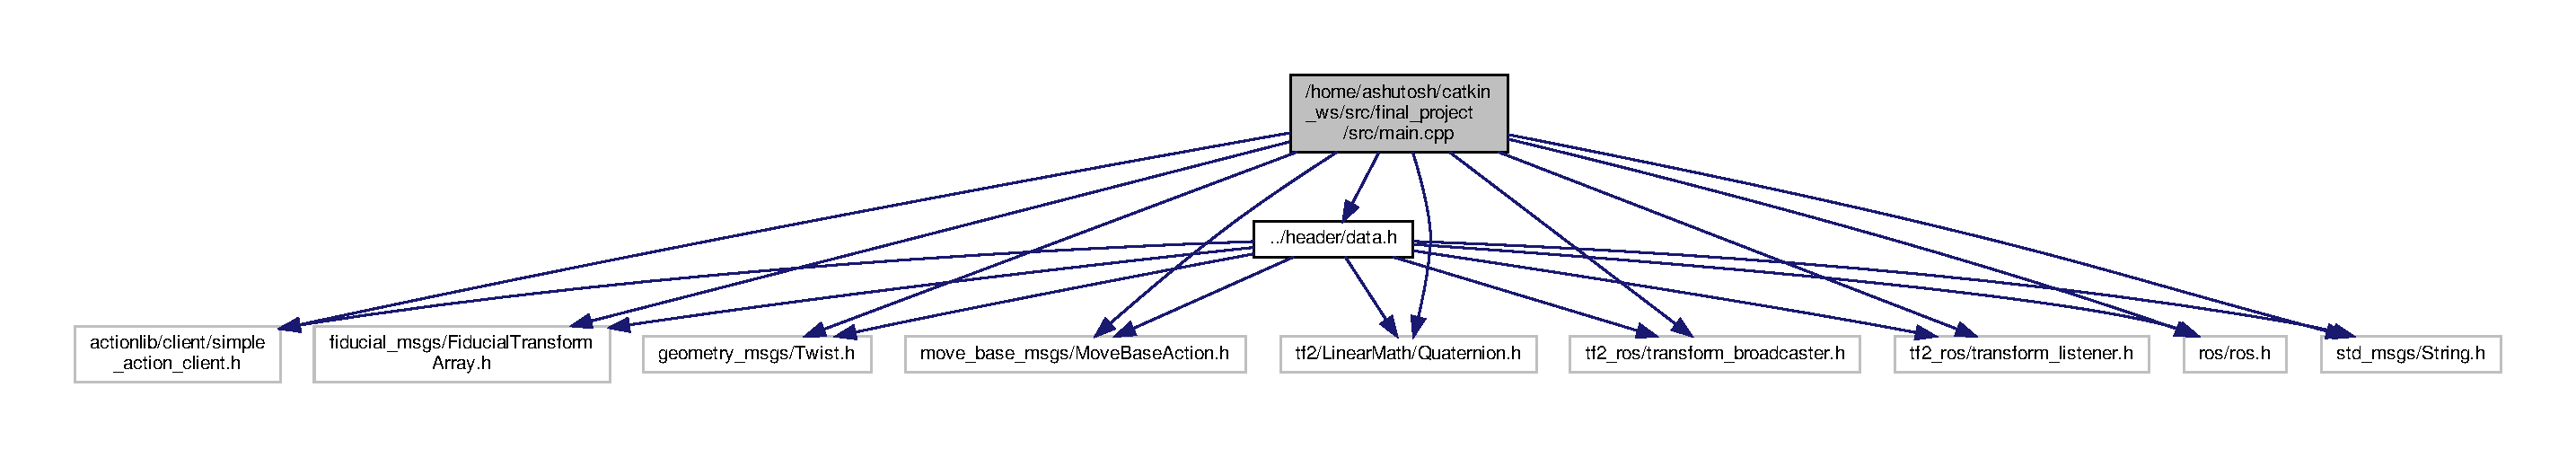
\includegraphics[width=350pt]{main_8cpp__incl}
\end{center}
\end{figure}
\subsection*{Functions}
\begin{DoxyCompactItemize}
\item 
void \hyperlink{main_8cpp_aef65d976146cab1c9987f30e9c49c6f8}{fiducial\+\_\+callback} (const fiducial\+\_\+msgs\+::\+Fiducial\+Transform\+Array\+::\+Const\+Ptr \&msg)
\begin{DoxyCompactList}\small\item\em function used to find aruco marker data \end{DoxyCompactList}\item 
\mbox{\Hypertarget{main_8cpp_a299d89c50484c4d3a597f6b43b65e21c}\label{main_8cpp_a299d89c50484c4d3a597f6b43b65e21c}} 
void \hyperlink{main_8cpp_a299d89c50484c4d3a597f6b43b65e21c}{broadcast} ()
\begin{DoxyCompactList}\small\item\em Function used to collect data from camera frame. \end{DoxyCompactList}\item 
void \hyperlink{main_8cpp_a1cb8c936ae579242b9f9fe4f9d172e73}{listen} (tf2\+\_\+ros\+::\+Buffer \&tf\+Buffer, double x, double y)
\begin{DoxyCompactList}\small\item\em Function used to map follower path in aruco marker order. \end{DoxyCompactList}\item 
\mbox{\Hypertarget{main_8cpp_a3c04138a5bfe5d72780bb7e82a18e627}\label{main_8cpp_a3c04138a5bfe5d72780bb7e82a18e627}} 
int {\bfseries main} (int argc, char $\ast$$\ast$argv)
\end{DoxyCompactItemize}


\subsection{Detailed Description}
The aim of the project is Urban Search \& Rescue by executing the individual tasks of navigating the explorer and follower robots in the given map. 

\begin{DoxyAuthor}{Authors}
Sri Sai Charan Velisetti (\href{mailto:svellise@umd.edu}{\tt svellise@umd.\+edu}), Mukundhan Rajendiran (\href{mailto:mrajeni@umd.edu}{\tt mrajeni@umd.\+edu}), Ashutosh Reddy Atimyala (\href{mailto:atimyala@umd.edu}{\tt atimyala@umd.\+edu}) 
\end{DoxyAuthor}
\begin{DoxyVersion}{Version}
0.\+1 
\end{DoxyVersion}
\begin{DoxyDate}{Date}
2021-\/12-\/15
\end{DoxyDate}
\begin{DoxyCopyright}{Copyright}
Copyright (c) 2021 
\end{DoxyCopyright}


\subsection{Function Documentation}
\mbox{\Hypertarget{main_8cpp_aef65d976146cab1c9987f30e9c49c6f8}\label{main_8cpp_aef65d976146cab1c9987f30e9c49c6f8}} 
\index{main.\+cpp@{main.\+cpp}!fiducial\+\_\+callback@{fiducial\+\_\+callback}}
\index{fiducial\+\_\+callback@{fiducial\+\_\+callback}!main.\+cpp@{main.\+cpp}}
\subsubsection{\texorpdfstring{fiducial\+\_\+callback()}{fiducial\_callback()}}
{\footnotesize\ttfamily void fiducial\+\_\+callback (\begin{DoxyParamCaption}\item[{const fiducial\+\_\+msgs\+::\+Fiducial\+Transform\+Array\+::\+Const\+Ptr \&}]{msg }\end{DoxyParamCaption})}



function used to find aruco marker data 


\begin{DoxyParams}{Parameters}
{\em msg} & \\
\hline
\end{DoxyParams}


Definition at line 267 of file main.\+cpp.

\mbox{\Hypertarget{main_8cpp_a1cb8c936ae579242b9f9fe4f9d172e73}\label{main_8cpp_a1cb8c936ae579242b9f9fe4f9d172e73}} 
\index{main.\+cpp@{main.\+cpp}!listen@{listen}}
\index{listen@{listen}!main.\+cpp@{main.\+cpp}}
\subsubsection{\texorpdfstring{listen()}{listen()}}
{\footnotesize\ttfamily void listen (\begin{DoxyParamCaption}\item[{tf2\+\_\+ros\+::\+Buffer \&}]{tf\+Buffer,  }\item[{double}]{x,  }\item[{double}]{y }\end{DoxyParamCaption})}



Function used to map follower path in aruco marker order. 


\begin{DoxyParams}{Parameters}
{\em tf\+Buffer} & \\
\hline
{\em x} & //\+Current postion of robot in x-\/axis \\
\hline
{\em y} & //\+Current postion of robot in y-\/axis \\
\hline
\end{DoxyParams}


Definition at line 63 of file main.\+cpp.


%--- End generated contents ---

% Index
\backmatter
\newpage
\phantomsection
\clearemptydoublepage
\addcontentsline{toc}{chapter}{Index}
\printindex

\end{document}
